The general idea behind this approach is simple: There exists one network which takes the futures' term structure as input and outputs a prediction of spread prices. If not specified otherwise the prices of the next business day are predicted. This is quite similar to figure~\ref{fig:longspread} where the green data points are the input and the blue data points -- but now for the next day! -- the output. Ideally one just has to find optimal hyperparameters.

The first part of this section will be about getting familiar with the data itself. This includes a general description as well as the handling of problematic data points.
Thereafter the network architecture as well as the tunable hyperparameters will be introduced more formally.
At last the the results of this approach are presented in a detailed manner.

\section{Data description and data handling}
\label{sec:aao-data-handling}

Primarily, the available data are the prices of VIX futures since they were first issued in 2004. Supplementary there is data about the VIX itself as well as additional information about the futures: their symbol and their precise date of expiration. All of these are sampled on a daily interval. There is also minutely data available which will not be used unless explicitly mentioned.

\subsection{Input data (term structure)}
\label{sec:aao-input-data}

The set of term structure data includes 3,304 samples in total from March 26th, 2004 to May 5th, 2017. Each term structure consists of three up to eight legs. The legs symbolize the months when the respective future expires. The specific date of expiration is always a workday in the middle of this month. For an example term structure see table~\ref{tab:single-termstructure} and for a graphical overview over the whole data set see figure~\ref{fig:termstructures}. Notice how similar the legs look to each other and to the VIX from figure~\ref{fig:vix}. To make the curvature between the term structures' legs more explicit their difference is calculated and used as network input.

\begin{table}
	\centering
	\caption[Single term structure with expiration dates (February 29th, 2012)]{A single term structure with expiration dates (February 29th, 2012) and corresponding long prices. The eight values are the futures' current prices for the next eight months. The expiration row shows the date the respective future expires. After expiration one can not invest in this future anymore.}
	\begin{tabular}{lllllllll}
	\toprule
	{} &      M1 &      M2 &      M3 &      M4 &      M5 &      M6 &      M7 &      M8 \\
	\midrule
	Value      &   21.00 &   23.99 &   25.60 &   26.50 &   27.75 &   28.40 &   29.05 &   29.25 \\
	Expiration &  Mar 21 &  Apr 18 &  May 16 &  Jun 20 &  Jul 18 &  Aug 22 &  Sep 19 &  Oct 17 \\
    \midrule	
    Long Price &         &    1.38 &    0.71 &   -0.35 &    0.60 &    0.00 &    0.45 &         \\
	\bottomrule
	\end{tabular}
 	\label{tab:single-termstructure}
\end{table}

\begin{figure}
	\centering
	\includegraphics[width=0.9\linewidth]{termstructures}
	\caption[Complete data set of term structures]{%
		Complete data set of term structures. Each term structure consists of at most eight legs (M1 to M8) where M1 is closest to expiration (blue). For most of the data -- except in times of crisis -- the legs with later expiration (green) have a higher price. Furthermore the general shape of the data is very similar between legs as well as similar to the VIX itself (see figure~\ref{fig:vix}).}
	\label{fig:termstructures}
\end{figure}

One problem for this task is missing data. If there are values for all eight months of a term structure like in table~\ref{tab:single-termstructure} this is a \emph{complete} sample. Consequently, when there are values missing it is an \emph{incomplete} sample. As seen in figure~\ref{fig:some-nice-graphics} there are especially many incomplete samples in earlier years. Because trading of futures just started it was not as established as of now. Futures are issued per month. But even though this happens regulary for each consecutive month since 2012 this was not always the case before. However, this regularity is necessary for a complete term structure. Removing all incomplete samples would shrink the dataset by $35\%$. 
By removing all samples before October 23th, 2006 only samples with up to two missing legs are left. This shrinks the data set by just $20\%$ resulting in 2,656 remaining samples. The remaining incomplete samples need to be handled by the network itself.

\begin{figure}
		\centering
	\begin{subfigure}{0.45\linewidth}
		\includegraphics[width=\linewidth]{number_of_samples}
		\caption{Number of samples by year}
		\label{fig:missing-values}
	\end{subfigure}
	\begin{subfigure}{0.45\linewidth}
		\includegraphics[width=0.95\linewidth]{missing_values}
		\caption{Distribution of missing values}
		\label{fig:weekdays}
	\end{subfigure}
	\caption[Number of samples by year and distribution of missing values]{%
		While a whole term structure consists of eight legs there is often less data available, especially in earlier years. Even though there are less samples from 2004 to 2006 there is a larger number of \emph{incomplete} term structures, often missing up to five legs.}
	\label{fig:some-nice-graphics}
\end{figure}

\subsection{Target data (long spread prices)}
\label{sec:aao-target-data}

For training a network one needs inputs as well as corresponding targets. While the term structure data set holds the necessary inputs, it is easy to calculate the target by applying \eqref{eq:long-spread} thus getting the long spread prices (see table~\ref{tab:single-termstructure}).\footnote{%
	Because of \eqref{eq:spread-correlation} it is sufficient to either calculate long spreads \emph{or} short spreads.}
For a complete term structure we get a complete set of spread prices consisting of six values.
Obviously the targets are the spread prices of the next term. Otherwise the network will not learn to make a prediction but an approximation of the applied formula. Because the term structure is the calculatory basis of the spread prices, they suffer from the same problem of missing data. Furthermore one has to exercise caution when expiration is close, so prediction is not made for already expired values.

\subsection{Seasonality}
\label{sec:seasonality}

As the original problem is finding inefficiencies in the term structure the network needs to be able to predict some recurring patterns. Therefore one might need some additional prior introducing seasonality. Some options are:

\newpage

\begin{itemize}
	\item The day of the month (1st to 31st)
	\item The month itself (Jan to Dec)
	\item The days until expiration of the term structure's first leg (0 to 34; see figure~\ref{fig:daystoexpiration})
\end{itemize}

The latter one -- the days until expiration -- has a nice property that is hopefully\footnote{%
Understanding what exactly a network actually learns is very difficult. One can not simply assume the same behavior as for humans. Most of the time one can only \emph{hope} the own choices were correct.}
advantageous in this context: 
There exist a total order. The former two are categorical by nature, e.g. without knowing about the year, January is \emph{not smaller} than February. But it is certainly possible to count down the days until expiration. Therefore it is appropriate to model these as a simple natural number at the network's input. For the alternatives is might have been necessary to use more verbose representations like a one-hot vector.\footnote{%
	A \emph{one-hot vector} is a binary vector with the same length as there are classes. All entries are $0$, except one which holds the value $1$. The position of this $1$ denotes the corresponding class.}

\begin{figure}
	\centering
	\includegraphics[width=0.9\linewidth]{days_to_expiration}
	\caption[Distribution of days to expiration for the termstructures' first leg]{%
		Distribution of days to expiration for the term structures' first leg.}
	\label{fig:daystoexpiration}
\end{figure}

\begin{table}
	\centering
	\caption[Descriptive statistics for futures and spread prices]{Common descriptive statistics for futures, their legs' difference and spread prices.}
	\begin{tabular}{lrrrrrrr}
		\toprule
		{} &  Mean &  Std. &    Min. &   25\% &   50\% &   75\% &  Max. \\
		\midrule
		Futures & 22.38 & 6.91 &  10.24 & 17.55 & 20.70 & 25.70 & 67.90 \\
		Difference & 0.38 & 1.00 & 21.10 & 0.07 & 0.40 & 0.75 & 5.45 \\
		Spread prices  &  0.11 & 0.74 & -13.68 & -0.10 &  0.13 &  0.36 &  4.90 \\
		\bottomrule
	\end{tabular}
	\label{tab:descriptive-stats}
\end{table}

\subsection{Normalization}

Looking at the most common descriptive statistics for input and target data in table~\ref{tab:descriptive-stats} -- especially the quantiles -- the spread prices are usually smaller than the futures by two orders of magnitude. And even for the differences of the futures' legs there are some outliers. This will not necessarily pose a problem but nevertheless \emph{optional} normalization is introduced by:

\begin{equation}
	X' = \frac{X - \bar{X}}{X_{max} - X_{min}} \quad \text{where $\bar{X}$ is the mean.}
\end{equation}

Hence, the resulting values of $X'$ will be in range $[0,1]$.

When explicitly mentioned am alternative formula for normalization is used, leading to zero mean and unit variance:

\begin{equation}
	\label{eq:normalization2}
	X'' = \frac{X - \bar{X}}{Std(X)} = \frac{X - \bar{X}}{\sqrt{Var(X)}}
\end{equation}

\subsection{Validation and test set}
\label{sec:aao-validation-and-test-set}

For validating the performance of deep networks the most widespread approach is to use one part of the data for tuning the hyperparameters introduced in section~\ref{sec:hyperparameters} (the \emph{validation set}) and one part for evaluating the final model (the \emph{test set}). In this work $15\%$ of the data will be used for validation and test set each. 

Looking at figure~\ref{fig:termstructures} it becomes evident that there is a temporal connection between areas of low and high price: If you look at some sample with low priced futures there is a high probability that samples next to this one also have a low price and vice versa. Therefore choosing completely random samples for validation and testing will result in datasets highly similar to the training set. But choosing one large connected chunk will result in hyperparameters fitted only to this timeframe. Choosing a tradeoff, test and validation set will be chosen by taking two chunks of data from different locations of the original data each, as shown in figure~\ref{fig:validation-and-test-set}.

\begin{figure}
	\centering
	\includegraphics[width=0.9\linewidth]{images/validation-and-test-set}
	\caption[Splitting whole dataset into training, validation and test set]{Splitting the whole dataset into training, validation and test set. The top figure shows the futures' prices for the next eight months (M1 to M8) of expiration forming the term structure. The bottom figure shows the corresponding spread prices. While the green area shows the data used for validation the red area is used for testing. The remaining data is used for training.}
	\label{fig:validation-and-test-set}
\end{figure}


\section{Network architecture}
\label{sec:aao-network-architecture}

A feedforward neural network is one oft the simplest architectures used in deep learning. First, there will be some definitions describing the network as well as some intuitions about training of neural networks. Thereafter the hyperparameters for tailoring the network to the problem are introduced. To prevent clueless searching over all of these some defaults are adopted. Finally, as already mentioned, the network needs to handle missing data. Some simple approach introducing an additional layer at the networks' output is introduced.

\subsection{Definitions}

The feedforward neural network can formally be described as a sequence of matrix-vector multiplications. Let $L$ be the number of hidden layers where $l \in \{1,\dots,L\}$ is the hidden layer's index. For a layer $l$ there is an input vector $\mathbf{z}^{(l)}$, an output vector $\mathbf{y}^{(l)}$ as well as a weight matrix $W^{(l)}$ and a bias vector $\mathbf{b}^{(l)}$. The input layer be $\mathbf{x} = \mathbf{y}^{(0)}$ and the output $\mathbf{t} = \mathbf{y}^{(L+1)}$. Furthermore there is an activation function $f^{(l)}$. At the output $f^{(L+1)}$ is typically the identity function.

Inference is done by the following operations for $l \in \{1,\dots,L+1\}$:

\begin{align}
	\label{eq:layer-input}
	\mathbf{z}^{(l)} &= W^{(l)\top} \mathbf{y}^{(l-1)} + \mathbf{b}^{(l)} \\
	\label{eq:layer-output}
	\mathbf{y}^{(l)} &= f^{(l)}(\mathbf{z}^{(l)})
\end{align}

Each hidden layer can have an arbitrary width greater zero. A layer's width is the length of the vector $\mathbf{y}^{(l)}$. In this work each hidden layer has the same width. Let this be the network's width $K$. Accordingly, the number of hidden layers $L$ is the network's depth.

For training -- this corresponds to optimizing $W$ and $\mathbf{b}$ -- the \emph{back-propagation} algorithm along with an optimization method like \emph{stochastic gradient descent} is used. Therefore a scalar loss function $J(\mathbf{t}, \mathbf{\hat{t}})$ is introduced, comparing the output of the network $\mathbf{t}$ to the target $\mathbf{\hat{t}}$. By iteratively computing the gradient with respect to the parameters $W$ and $\mathbf{b}$ for $J$ as well as for the activation functions $f^{(l)}$ backwards through the network one can optimize each layer's parameters. For further details see \cite{Rumelhart-1986a} and \cite[p.\,204ff.]{Goodfellow-et-al-2016}.

\subsection{Hyperparameters}
\label{sec:hyperparameters}

These definitions result in a number of tunable hyperparameters, potentially affecting the network's performance:
\begin{itemize}
	\item Activation functions $f^{(l)}$
	\item Loss function $J$
	\item Optimization method (and corresponding hyperparameters)
	\item Weight initializations (choosing initial values for $W^{(l)}$)
	\item Network depth $L$
	\item Network width $K$
\end{itemize}

While for some of these it is relatively easy to find some good values or there is some reasonable default, others are highly dependent on the problem and the data. For these, one has to extensively search for optimal values while constantly validating the performance. 

\paragraph{Activation functions.}
(also called hidden units when used together with their input from \eqref{eq:layer-input}) \\
One can read in \cite[p.\,191]{Goodfellow-et-al-2016}:
\begin{quote}
	``The design of hidden units is an extremely active area of research and does not yet have many definitive guiding theoretical principles.''
\end{quote}

\begin{wrapfigure}[8]{r}{0.3\textwidth}
	\vspace{-1em}
	\fbox{%
		\begin{minipage}{0.3\textwidth}\centering
			\includegraphics[width=\textwidth]{images/rectifier}
			\vspace{-20pt}
			\caption[Rectifier function]{%
				Rectifier \\ function $f(z)=\max(0,z)$}
			\label{fig:rectifier}
	\end{minipage}}
\end{wrapfigure}

Although directly followed by:
\begin{quote}
	``Rectified linear units are an excellent default choice of hidden unit.''
\end{quote}

A \emph{rectified linear unit} (ReLU) uses the activation function $f(z)=\max(0,z)$ (also called \emph{rectifier}, see figure~\ref{fig:rectifier}) meaning for $z \leq 0$ it always outputs zero. This offers some nice and simple properties especially regarding its derivative.\footnote{%
	The derivative is 0 across half its domain and 1 in the other. Furthermore the second derivative is 0 almost everywhere eliminating second-order effects.}
Using this function should ensure reasonable performance.

An alternative might be using \emph{scaled exponential linear units} (SELUs) as activations thus building a \emph{self-normalizing neural network}.\cite{DBLP:journals/corr/KlambauerUMH17} This is a very recent approach aiming for mapping the mean and variance from each layer to the next one. They explicitly try to solve some shortcoming of feedforward neural networks, often showing effective regularization properties. The SELU activation function is given by:

\begin{equation}
	\label{eq:selu}
	f(z) = \lambda
	\begin{cases}
	z & \text{if } z > 0 \\
	\alpha e^z - \alpha & \text{if } z \leq 0
	\end{cases}
\end{equation}

The corresponding paper suggests using $\alpha = 1.6733$ and $\lambda = 1.0507$ implying zero mean and unit variance. These are most effective if the training data has zero mean and unit variance, too, which can be accomplished by normalization using equation~\eqref{eq:normalization2}.

\paragraph{Loss function.}
This can be chosen quite conservatively, too. To penalize larger derivations from the target value proportionally more the \emph{mean squared error} (MSE) is used:
\begin{equation}
	\label{eq:mse}
	J(\mathbf{t}, \mathbf{\hat{t}}) =
	\frac{1}{n} \sum_{i=1}^{n}(t_i - \hat{t}_i)^2 \quad
	\text{where } n \text{ is the length of vector } \mathbf{t}.
\end{equation}

\paragraph{Optimization method.}
Most of the time \emph{stochastic gradient descent} (SGD) or some extension is chosen. The general idea is to use the gradient $\nabla_{\theta}J(\theta)$ of a function $J$ with parameters $\theta$ to find the direction (in parameter space) with the steepest descent. By updating the parameters iteratively with small steps\footnote{%
	Typically some value $\tau < 1$ is chosen like $0.01$ or $0.001$.}
of size $\alpha$ one is guaranteed to find a local minimum:

\begin{equation}
	\theta^{(i+1)} = \theta^{(i)} - \alpha \nabla_{\theta}J(\theta^{(i)})
\end{equation}

This formula describes the general gradient descent algorithm. As for the stochastic part, one takes a specific number of samples from the dataset -- called the \emph{batch size} -- and updates the parameters after evaluating just this sample. In deep learning SGD is applied with respect to weights $W$ and bias $\mathbf{b}$ for loss and activation functions. Because of the non-convex structure of neural networks finding a local minimum (instead of a global one) is acceptable. In practice this works reasonably well.

In this work primary the \emph{Adam}\footnote{``\dots the name Adam is derived from adaptive moment estimation.''} algorithm is used.\cite{DBLP:journals/corr/KingmaB14} It shows faster convergence, in general as well as for some specific tests on the current problem. New hyperparameters $\beta_1$ and $\beta_2$ are introduced for estimating the first and second moments of the gradients respectively. \\ The following hyperparameter settings are used: $\alpha=0.001$, $\beta_1 = 0.9$, $\beta_2=0.999$ (the latter two following the original paper's recommendations) and batch size of 32.

\paragraph{Weight initializations.}
For the presented iterative optimization methods the weights $W^{(l)}$ need to be initialized in some way. As mentioned above the optimization of a neural network is a non-convex problem. Therefore the local minimum found depends on these initializations. There are two properties which are especially important when choosing an initialization strategy.

First and foremost the initialization needs to break symmetry between units:

\begin{quote}
	``If two hidden units with the same activation function are connected to the same inputs, then these units must have different initial parameters. If they have the same initial
	parameters, then a deterministic learning algorithm applied to a deterministic cost
	and model will constantly update both of these units in the same way.''\cite[p.\,301]{Goodfellow-et-al-2016}
\end{quote}

Since one generally wants for each unit to learn some different aspects of the given task this is the most important role of initialization. 

Secondly, since SGD is used for optimization, the weights are updated with a certain step size. A small step size indicates the assumption that the values after optimization are close to the initial values. Taking both of these properties into account, using a common probability distribution seems to be an obvious solution. This work uses the following uniform distribution suggested by \cite{pmlr-v9-glorot10a}:

\begin{equation}
	\label{eq:glorot-initialization}
	W_{ij} \sim U\left[ -\frac{1}{\sqrt{k}}, \frac{1}{\sqrt{k}} \right]
	\quad \text{where $k$ is the width of the previous layer.} 
\end{equation}


\paragraph{Network depth and network width.}
Intuitively the network width increases the amount of information the network can ``remember''. The weight matrices are larger and therefore hold more values. Whereas the network depth increases the network's ability to learn underlying abstractions. A naive solution might be to chose width \emph{and} depth as large as possible. Unfortunately, this approach has serious drawbacks:

\begin{enumerate}
	\item One gets a powerful model which easily leads to overfitting\footnote{%
		This is a general problem in machine learning not limited to neural networks.}.
	The network will not learn to solve the problem but just echo its training. For samples outside the training set the performance will degrade drastically. This can distort the results in such a dramatic manner that some practitioners like \cite[p.\,23: When not to Backtest a Strategy]{Chan-2013} refuse to look at such models completely. One can fight overfitting by carefully choosing an out-of-sample validation set and using different kinds of regularization.
	
	\item As shortly explained above, the backpropagation algorithm uses the gradients for updating the weights backwards throughout the network. This may lead to the \emph{vanishing gradient problem} where the layers near the outputs are updated much faster than the layers near the inputs. Even though (very) deep networks were quite successful one some tasks during the recent years\footnote{%
		The ResNet architecture is very popular in image recognition. With a depth of 152 layers it even won 1st place on the Large Scale Visual Recognition Challenge (ILSVRC) 2015 classification task.\cite{DBLP:journals/corr/HeZRS15}}
	there is still no general solution for this problem, especially for feedforward networks.
	
	\item One may wish to force the network to learn abstractions and therefore require a certain depth. But a large depth in combination with a large width will not lead to the desired results because the network will likely use its many parameters to just ``remember'', ignoring the possibilities for abstraction coming with the additional hidden layers and therefore rendering them useless.
\end{enumerate}

There are some recent insights that imply using a powerful model with many parameters generally works well in deep learning.\cite{DBLP:journals/corr/ZhangBHRV16} But ultimately it comes down to the actual performance on the problem at hand. Therefore depth and width of the network will be considered tunable hyperparameters, too, that need to be evaluated empirically.

\subsection{Handling missing values at network level}

Up to now was a description of a standard feedforward architecture. In section~\ref{sec:aao-data-handling} the problem of missing data for inputs as well as outputs was described. These need to be handled partly by the network. At the inputs one can just set the missing values to zero. By looking at \emph{dropout regularization} one can see why this works. Here, the general idea is to randomly remove units during training to prevent them from co-adapting too much making each individual unit more robust eventually. This is implemented by adjusting the layers' input \ref{eq:layer-input} the following way: \cite{JMLR:v15:srivastava14a}

\begin{align}
	\mathbf{z}^{(l)} &= W^{(l)\top} \mathbf{\tilde{y}}^{(l-1)} + \mathbf{b}^{(l)} \\
	\text{where} \quad
	\mathbf{\tilde{y}}^{(l)} &= \underset{\text{entrywise product}}{\mathbf{r}^{(l)} \circ \mathbf{y}^{(l)}}
\end{align}

The values of vector $\mathbf{r}^{(l)}$ are from a Bernoulli distribution meaning $\mathbf{r}^{(l)} \in \{0, 1\}^k$.

Therefore by setting the inputs $\mathbf{y}^{(0)}$ not randomly but deterministically to zero -- in case they were missing in the first place -- the respective input nodes are effectively removed. It is important to note that this will not work for SELU activations because these do not settle at zero. Setting the inputs to $\lim_{z \to -\infty} f(z) = -\lambda \alpha$ might be a slightly better fit but is not really removing the corresponding input nodes.

For partly handling the outputs, missing values were set to zero and a conditional mask layer was added to the end of the network. The mask layer uses days to expiration as additional input: If this value is zero, the output for the spread price is set to zero, too. Both output and target would be zero resulting in $J(0, 0) = 0$. Because one does not know beforehand about the availability of the next term's data there is no way to handle the output in general.

The resulting architecture is illustrated in figure~\ref{fig:architecture1}.

\begin{figure}
	\centering
	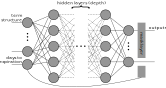
\includegraphics[width=0.9\linewidth]{architecture1}
	\caption[Network architecture with hidden layer width $K=5$]{%
		Network architecture with hidden layer width $K=5$. The mask layer just masks the first output in case there are zero days to expiration.}
	\label{fig:architecture1}
\end{figure}

\section{Evaluation}

Training a neural network to estimate a real valued vector comes down to a regression problem. This section is mainly about evaluating this chapter's approach for different configurations of hyperparameters.

\subsection{Network width, depth and normalization}

\begin{figure}
	\centering
	\begin{subfigure}{0.49\linewidth}
		\includegraphics[width=\linewidth]{approach1-ex1-loss-basic}
		\caption{}
	\end{subfigure}
	\begin{subfigure}{0.49\linewidth}
		\includegraphics[width=\linewidth]{approach1-ex1-val-basic}
		\caption{}
	\end{subfigure}
	\\
	\begin{subfigure}{0.49\linewidth}
		\includegraphics[width=\linewidth]{approach1-ex1-loss-normal}
		\caption{}
	\end{subfigure}
	\begin{subfigure}{0.49\linewidth}
		\includegraphics[width=\linewidth]{approach1-ex1-val-normal}
		\caption{}
	\end{subfigure}
	\caption[Resulting loss depending on width, depth and normalization]{The resulting loss depending on width, depth and normalization of training data. (a) Training loss without normalization; (b) Validation loss without normalization; (c) Training loss with normalization; (d) Validation loss with normalization.}
	\label{fig:approach1-ex1}
\end{figure}

\begin{figure}
	\centering
	\includegraphics[width=0.9\linewidth]{approach1-ex1-progression}
	\caption[Progression of training loss for networks with $L=1$ and $K=24$]{Progression of training loss for networks with $L=1$ and $K=24$. Mean and standard derivation (std.) over ten identical networks trained separately.}
	\label{fig:approach1-ex1-progression}
\end{figure}

For evaluating depth $L$ and width $K$ of the network as well as the influence of normalization a number of models different in these hyperparameters were trained. While the choice for normalization is a binary one, $L \in \{1,3,\dots,9\}$ and $K \in \{9,12,\dots,24\}$ were used. The training happened for 1,000 epochs\footnote{%
	One epoch specifies the number of iterations during SGD until the network as seen each sample exactly one time. For 1,000 epochs the network has seen each sample 1,000 times, subsequently.}
and for each combination ten models are trained to get information about mean and variance. A total of $2 \cdot 5 \cdot 6 \cdot 10 = 600$ models were trained.

For evaluating the results, for each model the epoch with the minimum loss was selected. Afterwards the mean over all models with identical hyperparameters was taken forming the figures in~\ref{fig:approach1-ex1}. There are three observations:

\begin{enumerate}
	\item As expected, the training loss decreases for more powerful models with larger depth and width. In contrast, the structure of the validation loss looks different. This is an example of overfitting where the network is not fitted to the problem but the training data only.
	\item Just looking at the validation loss, the performance obviously worsens with increasing depth. Only increasing the width seems to have an influence on decreasing the loss. These are similar results to \cite{Niaki-2013}.
	\item There is no obvious advantage to using normalized data. Looking at figure~\ref{fig:approach1-ex1-progression}, the network in general converges faster using normalized data but also shows higher variance. The differences are neglectable, therefore normalization is not pursued further.
\end{enumerate}


\subsection{Regularization techniques}

\begin{quote}
	``Many strategies	used in machine learning are explicitly designed to reduce the test error, possibly at the expense of increased training error. These strategies are known collectively as regularization.''\cite[p.\,228]{Goodfellow-et-al-2016}
\end{quote}

Regularization is especially important in deep learning, where it is hard to visualize and understand what exactly was learned by the network. There is a large number of regularization techniques available, some of them exclusive for neural networks. Even a simple strategy like ``stopping the training when the validation error increases'' (\emph{early stopping}) is already some kind of regularization. This section mainly focuses on comparing three approaches: The widespread \emph{dropout regularization}, \emph{self-normalizing neural networks} (using SELUs as activation functions) and an attempt on \emph{data augmentation}, using minutely data for training.\footnote{%
	Data augmentation: Creating similar -- but not identical -- data from existing one, increasing the variance and hence making the network more robust. Even though the data was not newly generated the general idea is similar. By using some minute's futures as input, targeting the spread prices of the same minute at the next term, the network would learn a similar mapping. The number of samples increases by factor 1,440.}

\begin{figure}
	\centering
	\begin{subfigure}{0.49\linewidth}
		\includegraphics[width=\linewidth]{approach1-ex3-val-minutely}
		\caption{}
	\end{subfigure}
	\begin{subfigure}{0.49\linewidth}
		\includegraphics[width=\linewidth]{approach1-ex3-val-selu}
		\caption{}
	\end{subfigure}
	\caption[Validation loss for models trained with regularization techniques]{Validation loss for models trained with (a) minutely data and (b) SELU activations.}
	\label{fig:approach1-ex3}
\end{figure}

For evaluating the effectiveness of regularization the range of width $K$ and especially depth $L$ to search over was widened, except for minutely data. Using $L \in \{1,4,\dots,91\}$ and $K \in \{3,6,\dots,33\}$ a total of $30 \cdot 30 = 900$ models were trained. The large raise of the maximum depth was done in hope of finding a network with better abstraction capabilities, since the former experiments favored shallow networks. There was only one training run per model configuration, therefore neglecting statistical soundness. 

For minutely data $L \in \{1, 4, \dots, 28\}$ and $K \in \{3,6,\dots,30\}$ were chosen. Further increasing the depth would have been computationally expensive. Because of similar reasons the batch size was set to 1024, also reducing the noise at each weight update. For each such configurations ten models were trained.

Looking at the results in figure~\ref{fig:approach1-ex3}, their implications do not seem much different from the former experiments. Again, for each model the epoch with minimum loss was selected:

\begin{enumerate}
	\item For dropout, the smallest loss was around $0.2$, much higher than all other models. Hence using dropout seems out of question. It neither allows for deeper networks nor does it result in an acceptable loss, regardless of configuration.
	\item Building self-normalizing neural networks with SELUs seems promising. But comparison with figure~\ref{fig:approach1-ex1} shows not much difference, concluding that in this case simple width is more important than some additional regularizations.
	\item Again, a small depth in connection with a large width seems to be the preferred configuration. 
\end{enumerate}

\subsection{Additional inputs}

Remembering section~\ref{sec:seasonality}, there were some additional inputs which might hold important information. Adding these inputs to the existing models might decrease the loss under the conditions that these features indeed are useful and that the model is able to learn their underlying pattern. 

Therefore two inputs are added: The corresponding day of month and the month itself, represented as simple natural numbers where January $\mapsto 1$, \dots, December $\mapsto 12$. Increasing the depth hurt performance in previous experiments, therefore depth $L = 1$ is chosen while width is set to $K \in \{20,23,\dots,50\}$. For each configuration ten models were trained, resulting in a total of $11 \cdot 10 = 110$ models. Furthermore, there were some training runs with normalized values but since the performance was always much worse these will not be evaluated further.

\begin{figure}[h!]
	\centering
	\includegraphics[width=0.9\linewidth]{approach1-ex4-val-basic}
	\caption[Validation loss using additional inputs with respect to width]{Validation loss for models with additional input. The x-axis shows the networks' width. Ten models were trained, shown by the thin lines. The thick blue line is the mean and the light blue area the standard derivation in either direction.}
	\label{fig:approach1-ex4}
\end{figure}

\newpage

The results are shown in figure~\ref{fig:approach1-ex4}. While mean and standard derivation seem reasonable, the loss itself only gains significance by comparing it to the other experiments. This is done in the following section.

\subsection{Comparison}
\label{sec:aao-comparison}

There are four models used for comparison, corresponding to the experiments described above:

\begin{enumerate}
	\item Basic network as presented in section~\ref{sec:aao-network-architecture} (Basic)
	\item Network using dropout regularization (Dropout)
	\item Self-normalizing network using SELUs (SNN)
	\item Basic network trained with minutely data (Minutely)
	\item Network with additional inputs for days and month (AddIn)
\end{enumerate}

All these networks have a depth $L=1$ and width $K=30$. Using a greater width might lead to marginally better performance. The training data is not normalized. Furthermore the learning rate is reduced by $\sqrt{0.1}$ up to two times if there is no improvement on the validation loss for 20 epochs. If there is still no improvement afterwards the training is stopped (\emph{early stopping}). As a baseline a naive prediction is used: It just assumes the futures' prices did not change for the next day, calculating spread prices and error from these.

By looking at table~\ref{tab:aao-comparison} -- especially the last column using the test dataset not used for network optimization -- the results are quite devastating. The error on most models is worse than for naive prediction. Only the self-normalizing network and the network trained with minutely data beat this by a negligible difference. Furthermore the training error is unusually high, often above the validation MSE. Even though the training data seems to have higher fluctuations -- likely because of the financial crisis in 2008 -- one could expect the networks to fit more to this dataset. Therefore this chapter's approach failed to deliver useful predictions.

\begin{table}
	\centering
	\caption[Comparison of the results obtained by the first approach]{Comparison of the results obtained by the first approach. Smaller error (MSE) indicated better performance. Because training and validation set were used for optimization the test MSE is most meaningful.}
	\begin{tabular}{llrrr}
		\toprule
		{} & Epoch &  Training MSE &  Validation MSE &  \textbf{Test MSE} \\
		\midrule
		Naive    &       &        0.2099 &          0.0985 &    0.1318 \\
		Basic    &   307 &        0.1386 &          0.1013 &    0.1563 \\
		Dropout  &   174 &        0.1895 &          0.2426 &    0.2984 \\
		SNN      &   242 &        0.1425 &          0.1077 &    \textbf{0.1259} \\
		Minutely &    70 &        0.2252 &          \textbf{0.0896} &    0.1294 \\
		AddIn    &   268 &        \textbf{0.1297} &          0.0997 &    0.1321 \\
		\bottomrule
	\end{tabular}
	\label{tab:aao-comparison}
\end{table}